\documentclass[11pt,a4paper]{article}
\usepackage[margin=2.5cm]{geometry}
\usepackage[T1]{fontenc}
\usepackage{amsmath,amssymb}
\usepackage{graphicx}
\usepackage{booktabs}
\usepackage[round]{natbib}
\usepackage[hidelinks]{hyperref}

% Replace the title, author and date.
\title{Tree Canopy and Summer Surface Temperature:\\A Field Study of 21 Neighbourhoods}
\author{Sofia Lindqvist\thanks{Department of Geography, Vestby University. Email: \texttt{sofia.lindqvist@vestby.example}}
\and Kwame Mensah\thanks{City Planning Office, Municipality of Vestby.}}
\date{March 2026}

\begin{document}
\maketitle

% Replace with your abstract.
\begin{abstract}
Cities are warmer than their surroundings, and the difference is largest on summer afternoons, when it matters most for health. Planting trees is the most common response, but how much cooling a given amount of canopy delivers is rarely measured locally. We measured surface temperature and tree canopy cover in 21 neighbourhoods of a mid-sized northern city during July 2025. Surface temperature fell by 0.23\,\textdegree C for every additional percentage point of canopy cover, and canopy explained 96\% of the variation between neighbourhoods. The relationship held for both residential and mixed-use areas. Raising canopy cover in the five least-shaded neighbourhoods to the city average would lower their afternoon surface temperature by an estimated 3.9\,\textdegree C.
\end{abstract}

\section{Introduction}\label{sec:introduction}
Paved and built surfaces absorb sunlight and release it as heat, so that dense urban areas are warmer than nearby countryside. The effect has been documented for two centuries and reviewed many times \citep{oke1982energetic,arnfield2003two}. Its consequences are uneven: neighbourhoods with little vegetation are hotter, and they are often the ones whose residents are least able to avoid the heat.

Trees cool their surroundings by shading surfaces and by evaporating water. \citet{bowler2010urban} reviewed the evidence and found that parks are on average about one degree cooler than non-green sites during the day, but they also noted that most studies compare a park with its surroundings rather than measuring canopy across ordinary streets. City planners, who decide where street trees go, need the second kind of evidence.

This article reports such a measurement. We ask how afternoon surface temperature varies with tree canopy cover across the neighbourhoods of one city, and what that implies for a planting programme. Section~\ref{sec:methods} describes the data, Section~\ref{sec:results} the results, and Section~\ref{sec:discussion} their limits.

\section{Data and Methods}\label{sec:methods}
\subsection{Study Area}
Vestby has 180\,000 inhabitants and a humid continental climate, with a mean July maximum of 23\,\textdegree C. We selected 21 neighbourhoods of between 0.4 and 1.1 square kilometres to cover the range of building density in the city. Fourteen are residential and seven are mixed-use.

\subsection{Measurements}
Canopy cover was estimated from aerial photographs taken in June 2025, as the share of each neighbourhood's area covered by tree crowns. Surface temperature was derived from three cloud-free satellite passes in July 2025, each at about 14:30 local time, and averaged per neighbourhood.

\subsection{Model}
We describe the relationship with a linear model,
\begin{equation}\label{eq:model}
  T_i = \beta_0 + \beta_1 C_i + \varepsilon_i ,
\end{equation}
where $T_i$ is the mean surface temperature of neighbourhood $i$ in degrees Celsius, $C_i$ its canopy cover in percent, and $\varepsilon_i$ an error term. The coefficient $\beta_1$ is the change in temperature per percentage point of canopy. We estimate \eqref{eq:model} by ordinary least squares.

\section{Results}\label{sec:results}
Canopy cover ranged from 4\% to 56\%, and surface temperature from 31.9 to 43.8\,\textdegree C. Figure~\ref{fig:scatter} shows the two together. The fitted line has an intercept of 44.6\,\textdegree C and a slope of $-0.23$\,\textdegree C per percentage point, with $R^2 = 0.96$.

\begin{figure}[htbp]
  \centering
  % Replace with your own figure: upload an image and change the file name below.
  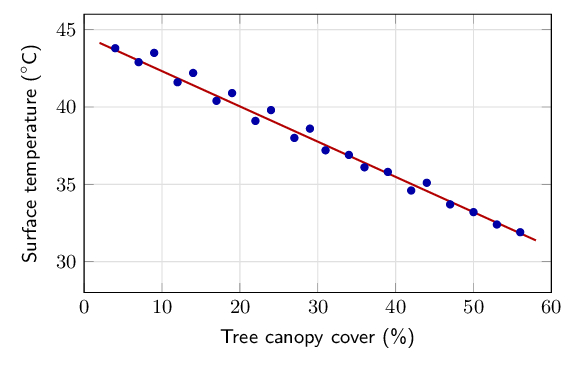
\includegraphics[width=0.75\textwidth]{figures/canopy-temperature.png}
  \caption{Afternoon surface temperature against tree canopy cover in 21 neighbourhoods, with the fitted line from Equation~\eqref{eq:model}.}
  \label{fig:scatter}
\end{figure}

Table~\ref{tab:groups} splits the neighbourhoods by land use. Mixed-use areas have less canopy and are warmer, but the slope is similar in both groups, which suggests that the cooling per unit of canopy does not depend strongly on building type.

\begin{table}[htbp]
  \centering
  \caption{Canopy cover, surface temperature and fitted slope by land use.}
  \label{tab:groups}
  \begin{tabular}{lcccc}
    \toprule
    Land use & Neighbourhoods & Mean canopy & Mean temperature & Slope \\
             &                & (\%)        & (\textdegree C)  & (\textdegree C per point) \\
    \midrule
    Residential & 14 & 33.6 & 36.9 & $-0.22$ \\
    Mixed-use   &  7 & 16.4 & 41.0 & $-0.25$ \\
    \midrule
    All         & 21 & 27.9 & 38.3 & $-0.23$ \\
    \bottomrule
  \end{tabular}
\end{table}

The five neighbourhoods with the least canopy average 10.8\% cover. Raising them to the city mean of 27.9\% would, by Equation~\eqref{eq:model}, lower their surface temperature by $0.23 \times 17.1 \approx 3.9$\,\textdegree C.

\section{Discussion}\label{sec:discussion}
The slope we find is steeper than most values reported for parks \citep{bowler2010urban}, which is expected: surface temperature responds more strongly to shade than air temperature does. The result should not be read as the cooling that residents would feel. It is, however, the quantity that determines how much heat pavements and walls store and release in the evening.

Three limits apply. The study covers one city and one month. Canopy cover is correlated with building density, so some of the effect may belong to density rather than to trees. And new trees take fifteen to twenty years to reach the crown size that the aerial photographs record.

\section{Conclusion}\label{sec:conclusion}
Across 21 neighbourhoods of Vestby, each additional percentage point of tree canopy was associated with a 0.23\,\textdegree C lower afternoon surface temperature in July. The relationship was strong, close to linear and similar for residential and mixed-use areas. Planting in the least-shaded neighbourhoods offers the largest reduction per tree.

\section*{Acknowledgements}
We thank the Vestby parks department for the aerial photographs and Ingrid Solberg for help with the canopy classification.

\bibliographystyle{plainnat}
\bibliography{references}

\end{document}
